% This is "sig-alternate.tex" V2.1 April 2013
% This file should be compiled with V2.8 of "sig-alternate.cls" May 2012
%
% This example file demonstrates the use of the 'sig-alternate.cls'
% V2.8 LaTeX2e document class file. It is for those submitting
% articles to ACM Conference Proceedings WHO DO NOT WISH TO
% STRICTLY ADHERE TO THE SIGS (PUBS-BOARD-ENDORSED) STYLE.
% The 'sig-alternate.cls' file will produce a similar-looking,
% albeit, 'tighter' paper resulting in, invariably, fewer pages.
%
% ----------------------------------------------------------------------------------------------------------------
% This .tex file (and associated .cls V2.8) produces:
%       1) The Permission Statement
%       2) The Conference (location) Info information
%       3) The Copyright Line with ACM data
%       4) NO page numbers
%
% as against the acm_proc_article-sp.cls file which
% DOES NOT produce 1) thru' 3) above.
%
% Using 'sig-alternate.cls' you have control, however, from within
% the source .tex file, over both the CopyrightYear
% (defaulted to 200X) and the ACM Copyright Data
% (defaulted to X-XXXXX-XX-X/XX/XX).
% e.g.
% \CopyrightYear{2007} will cause 2007 to appear in the copyright line.
% \crdata{0-12345-67-8/90/12} will cause 0-12345-67-8/90/12 to appear in the copyright line.
%
% ---------------------------------------------------------------------------------------------------------------
% This .tex source is an example which *does* use
% the .bib file (from which the .bbl file % is produced).
% REMEMBER HOWEVER: After having produced the .bbl file,
% and prior to final submission, you *NEED* to 'insert'
% your .bbl file into your source .tex file so as to provide
% ONE 'self-contained' source file.
%
% ================= IF YOU HAVE QUESTIONS =======================
% Questions regarding the SIGS styles, SIGS policies and
% procedures, Conferences etc. should be sent to
% Adrienne Griscti (griscti@acm.org)
%
% Technical questions _only_ to
% Gerald Murray (murray@hq.acm.org)
% ===============================================================
%
% For tracking purposes - this is V2.0 - May 2012

\documentclass{sig-alternate}



\begin{document}

% Copyright
\setcopyright{waclicense}


%% DOI
%\doi{10.475/123_4}
%
%% ISBN
%\isbn{123-4567-24-567/08/06}
%
%%Conference
%\conferenceinfo{PLDI '13}{June 16--19, 2013, Seattle, WA, USA}
%
%\acmPrice{\$15.00}

%
% --- Author Metadata here ---
\conferenceinfo{Web Audio Conference WAC-2016,}{April 4--6, 2016, Atlanta, USA}
\CopyrightYear{2016} % Allows default copyright year (20XX) to be over-ridden - IF NEED BE.
%\crdata{0-12345-67-8/90/01}  % Allows default copyright data (0-89791-88-6/97/05) to be over-ridden - IF NEED BE.
% --- End of Author Metadata ---

\title{Time Stretching \& Pitch Shifting with Web Audio API: Where are we at?}
%\subtitle{[Extended Abstract]
%\titlenote{A full version of this paper is available as
%\textit{Author's Guide to Preparing ACM SIG Proceedings Using
%\LaTeX$2_\epsilon$\ and BibTeX} at
%\texttt{www.acm.org/eaddress.htm}}}
%
% You need the command \numberofauthors to handle the 'placement
% and alignment' of the authors beneath the title.
%
% For aesthetic reasons, we recommend 'three authors at a time'
% i.e. three 'name/affiliation blocks' be placed beneath the title.
%
% NOTE: You are NOT restricted in how many 'rows' of
% "name/affiliations" may appear. We just ask that you restrict
% the number of 'columns' to three.
%
% Because of the available 'opening page real-estate'
% we ask you to refrain from putting more than six authors
% (two rows with three columns) beneath the article title.
% More than six makes the first-page appear very cluttered indeed.
%
% Use the \alignauthor commands to handle the names
% and affiliations for an 'aesthetic maximum' of six authors.
% Add names, affiliations, addresses for
% the seventh etc. author(s) as the argument for the
% \additionalauthors command.
% These 'additional authors' will be output/set for you
% without further effort on your part as the last section in
% the body of your article BEFORE References or any Appendices.

\numberofauthors{3} %  in this sample file, there are a *total*
% of EIGHT authors. SIX appear on the 'first-page' (for formatting
% reasons) and the remaining two appear in the \additionalauthors section.
%
%\author{
% You can go ahead and credit any number of authors here,
% e.g. one 'row of three' or two rows (consisting of one row of three
% and a second row of one, two or three).
%
% The command \alignauthor (no curly braces needed) should
% precede each author name, affiliation/snail-mail address and
% e-mail address. Additionally, tag each line of
% affiliation/address with \affaddr, and tag the
% e-mail address with \email.
%
% 1st. author
%\alignauthor Matthew E. P. Davies
%	\affaddr{Sound and Music Computing Group, INESC TEC, Porto, Portugal}
%	\email{mdavies@inesctec.pt}
% 2nd. author
%\alignauthor David Martins Matos\\
%	\affaddr{INESC-ID, IST - Universidade de Lisboa, Portugal}\\
%       	\email{david.matos@inesc-id.pt }
% 3rd. author
%\alignauthor Helena Sofia Pinto\\
%	\affaddr{INESC-ID, IST - Universidade de Lisboa, Portugal}\\
%       	\email{sofia@ontol.inesc-id.pt }
%\and
% 4th. author
%\alignauthor Bruno Dias\\
%	\affaddr{INESC-ID, IST - Universidade de Lisboa, Portugal}\\
%      	\email{bruno.s.dias@ist.utl.pt}
%}

% There's nothing stopping you putting the seventh, eighth, etc.
% author on the opening page (as the 'third row') but we ask,
% for aesthetic reasons that you place these 'additional authors'
% in the \additional authors block, viz.
\date{1 September 2015}
% Just remember to make sure that the TOTAL number of authors
% is the number that will appear on the first page PLUS the
% number that will appear in the \additionalauthors section.

\maketitle
\begin{abstract}

Audio time stretching and pitch shifting are operations that all major commercial and/or open source Digital Audio Workstations, DJ Mixing Software and Live Coding Suites offer. Those operations allow users to change tempo while maintaining the pitch and vice-versa. Unfortunately, there are few (and experimental) client-side Javascript implementations of those two operations.

In this paper, we review the current state of art for client-side implementations of time stretching and pitch shifting, their limitations, and describe two new implementations for two well-known algorithms: (1) Phase Vocoder with Identity Phase Lock and (2) a modified version of Overlap \& Add.

Additionally, we discuss some issues related to Web Audio API (WAA) and Frequency-based audio process, regarding latency and audio quality in pitch shifting and hoping to raise awareness over some potential (and welcome) changes in WAA.
\end{abstract}


%
% The code below should be generated by the tool at
% http://dl.acm.org/ccs.cfm
% Please copy and paste the code instead of the example below. 
%
%\begin{CCSXML}
%<ccs2012>
 %<concept>
  %<concept_id>10010520.10010553.10010562</concept_id>
  %<concept_desc>Computer systems organization~Embedded systems</concept_desc>
  %<concept_significance>500</concept_significance>
 %</concept>
 %<concept>
  %<concept_id>10010520.10010575.10010755</concept_id>
  %<concept_desc>Computer systems organization~Redundancy</concept_desc>
  %<concept_significance>300</concept_significance>
 %</concept>
 %<concept>
  %<concept_id>10010520.10010553.10010554</concept_id>
  %<concept_desc>Computer systems organization~Robotics</concept_desc>
  %<concept_significance>100</concept_significance>
 %</concept>
 %<concept>
  %<concept_id>10003033.10003083.10003095</concept_id>
  %<concept_desc>Networks~Network reliability</concept_desc>
  %<concept_significance>100</concept_significance>
 %</concept>
%</ccs2012>  
%\end{CCSXML}
%
%\ccsdesc[500]{Computer systems organization~Embedded systems}
%\ccsdesc[300]{Computer systems organization~Redundancy}
%\ccsdesc{Computer systems organization~Robotics}
%\ccsdesc[100]{Networks~Network reliability}
%
%
%%
%% End generated code
%%
%
%%
%%  Use this command to print the description
%%
%\printccsdesc
%
%% We no longer use \terms command
%%\terms{Theory}
%
%\keywords{ACM proceedings, \LaTeX, text tagging}

\section{Introduction}

Time stretching and pitch shifting are two operations widely available in commercial and open source musical applications like Ableton Live\footnote{https://www.ableton.com/}, Traktor Pro\footnote{http://bit.ly/1izsxHy} and Ardour\footnote{http://ardour.org/}. Currently, creative frameworks implemented in JavaScript and Web Audio API (WAA) like Flocking \cite{flocking:icmc2014} and Tone.js \cite{tonejs:wac2015} only offer time stretching through re-sampling of audio buffers, changing both the duration (i.e.: tempo) and pitch at the same time. In digital audio workstations (DAW) like EarSketch \cite{earsketch:wac2015}, time stretching and pitch shifting is performed server-side, with SoX\footnote{http://sox.sourceforge.net/}, making real-time interaction impossible.

This paper presents an overview of the current implementations for both algorithms using JavaScript in the browser environment and two new implementations. Additionally, we discuss the impact of certain decisions in WAA design, and philosophy, regarding the absence of frequency-based operators, like Fast Fourier Transform (FFT), cause an impact in performance.

For both implementations, we had the following non-functional requirements: 
\begin{itemize}
	\item \textbf{Constant memory usage}, with fixed size circular arrays, in order to minimize the impact of the garbage collector, by maintaining a constant memory profile.
	\item \textbf{Intuitive API and documentation} because time stretching, for the current Web Audio API community, seems to be a difficult subject.
	\item \textbf{Minimize assumptions} regarding sample rate, number of channels and the type of audio (percussive or harmonic) being processed.
\end{itemize}

The outline of the paper is the following. First, we review the basic theory for time, and frequency, time stretch and pitch shifting algorithms. Then, we describe the existing Javascript implementations of such algorithms. After that, we present our two new implementations for two well know algorithms: (1) Phase Vocoder with Identity Phase Locking\cite{laroche:phasinessbusiness} and (2) a modified Overlap \& Add (OLA) algorithm. Finally, we discuss the trade-offs between existing implementations and problems with WAA regarding these two operations.

\section{Theoretical Background}

For both tasks, there are algorithms that work in time domain, like Overlap and Add (OLA) \cite{}, Waveform Similarity based OLA (WSOLA) \cite{verhelst:wsola93} and delay line modulation \cite{modulationline:pitchshift}, and others that work in the frequency domain, like the Phase Vocoder \cite{dolsontutorial:phasevocoder} and Spectral Modelling \cite{dafx:2nd}. In this section, we give an overview of three popular methods: OLA, WSOLA and Phase Vocoder.

\subsection{OLA}

Algorithms in both time and frequency domains, for Time Stretching and Pitch Shifting, are more sophisticated versions of OLA. There are three main steps for OLA:
\begin{enumerate}
	\item Chop the input signal into several (analysis) frames of size N, each overlapping with the previous one in $H_a$ (i.e.: the analysis hop size) samples.
	\item Apply a window to each analysis frame.
	\item Add the (synthesis) frame to the output, by overlapping it with $H_s$ (i.e.: the synthesis hop size) samples of the "tail" of the output signal.
\end{enumerate}
So, the main idea of OLA is to retrieve frames from the input signal, each one overlapping with consecutive input frames in $H_a$ samples, and overlapping each windowed input frame with the output signal, in $H_s$ samples. The relation between both overlap/hop sizes determines the stretching factor:

\begin{displaymath}
\alpha = \frac{H_s}{H_a}
\end{displaymath}

Usually, one of the hop sizes is fixed while the other is a function of $\alpha$. We should note that $\alpha$ can be change at each new frame. OLA does not preserve phase relations between consecutive frames and, as such, there are noticeable artefacts in the output signal: modulation of harmonic structures (e.g.: human voice) and reverberation. The temporal complexity of OLA is $O(N)$. In figure \ref{fig:ola}, it can be seen what happens to both $H_a$ and $H_s$ when changing the $\alpha$.
To perform pitch shifting with OLA, one could couple a re-sampler to the OLA time stretcher. In order to allow simultaneous time stretching and pitch shifting, let $\beta_{t}$ be the new desired pitch and $R_{t}$ the current sampling rate used in the re-sampler. Then, the new stretching factor $\alpha_{t+1}$ and the new sample rate $R_{t+1}$ are defined as 
\begin{displaymath}
\alpha_{t+1} = \frac{\alpha_{t}}{R_{t}}
\end{displaymath}
\begin{displaymath}
R_{t+1} = R_{t} * \beta_{t+1}
\end{displaymath}

\begin{figure}
	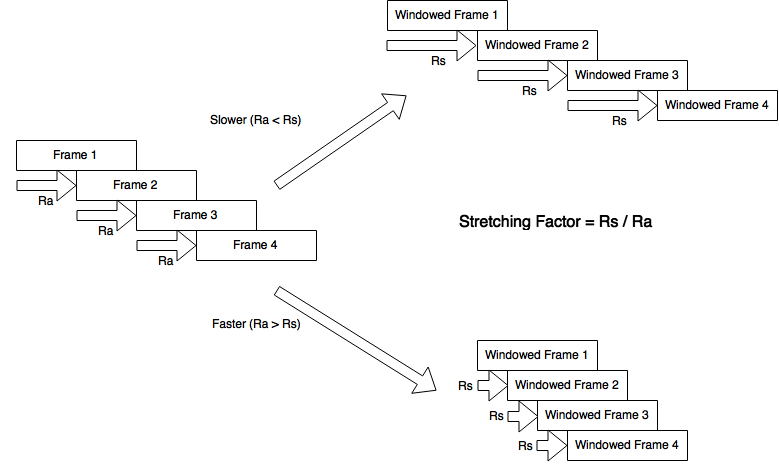
\includegraphics[width=3.5in]{ola}
	\caption{Example showing what happens, regarding hop sizes, for slowdowns and speed-ups of the audio.}
	\label{fig:ola}
\end{figure}

\subsection{WSOLA}

First introduced in \cite{verhelst:wsola93}, WSOLA applies a delay $\delta \in [-\delta_{max}:\delta_{max}]$ to each analysis frame, such that the waveforms of two overlapping synthesis frames are as similar as possible in the overlapping regions\footnote{WSOLA is equivalent to OLA when $\delta_{max}=0$.}. The delay can be obtained by calculating the cross-correlation between the overlapping regions of each synthesis sample. This algorithm removes the reverberation and modulation but, for transient rich sounds (percussion, guitar riffs), there might be some missing transients and stuttering (i.e.: repeated transients). Regarding the temporal complexity of WSOLA, if the cross-correlation is implemented with FFT Convolution \cite{dspguide}, we get $O(N log_2 N)$. Otherwise, if it is a "naive" implementation of the convolution, we get $O(N^2)$.
To perform pitch shifting, one can use the same method described for OLA.

\subsection{Phase Vocoder}

Phase Vocoder is a well documented \cite{dolsontutorial:phasevocoder,laroche:phasinessbusiness,dafx:2nd,phasevocoder:pitchshift,phasevocoder:bernardini,phavorit,phasevocoder:latency} algorithm used for Time Stretching \cite{dolsontutorial:phasevocoder,phavorit}, Pitch Shifting \cite{phasevocoder:pitchshift} and other audio effects like robotization \cite{dafx:2nd}. In general, it has higher computational costs than time domain methods like WSOLA but offers high quality audio, without missing transients. Each iteration of the Phase Vocoder has the following steps:
\begin{enumerate}
	\item Chop the input signal into several (analysis) frames of size N, each overlapping with the previous one in $H_a$ (i.e.: the analysis hop size) samples.
	\item Apply a window to each analysis frame.
	\item Calculate the forward Fourier Transform. TODO
	\item Calculate the magnitude and phase spectra of the frequency frame obtained in step 1. TODO
	\item Compute the phase difference between the current phase spectra and the previous one (i.e.: instantaneous frequency). TODO
	\item Calculate the difference between the instantaneous frequency and the centre frequency of each frequency bin. TODO
	\item Due to the fact that the phase values are given in modulo $2\pi$ and, as such, phase jumps will exists due to the nature of the polar representation, we need to calculate the principal determination of the difference obtained in the previous step. TODO
	\item Compute the Inverse Fourier Transform. TODO
	\item Add the (synthesis) frame to the output, by overlapping it with $H_s$ (i.e.: the synthesis hop size) samples of the "tail" of the output signal.
\end{enumerate}

This algorithm ensures \textit{horizontal phase coherence} (i.e.: phase continuity for the same frequency bin, in consecutive frequency frames) is guaranteed. However, \textit{vertical phase coherence} (i.e.: phase relations between different frequency bins, in the same frame) is usually destroyed in the phase correction process. The loss of \textit{vertical phase coherence} results in a distinct artefact: \textit{phasiness} (i.e.: metallic tunnel sound). The temporal complexity of the Phase Vocoder is $O(N\,log_{2}N)$.

To maintain both vertical and horizontal coherence, we can apply a technique known as \textit{Identity Phase-Locking} \cite{phasevocoder:identityphaselock}. The main idea is that frequency bins that are not spectral peaks contribute to the partials of the nearest spectral peak. In order to find the spectral peaks, one can use a simple heuristic: if a frequency bin has the maximum magnitude when compared with four neighbour bins,  then it is a spectral peak. After identifying all spectral peaks, we need to infer what is the "region of influence" of each peak (i.e.: for a given peak, what are the non-peak bins that contribute to the peak partial) (see section IIIC of \cite{phasevocoder:identityphaselock}). After identifying both the spectral peaks and the "regions of influence", the usual phase correction method is applied to the peak bins. The phase of a non-peak bin will be equal to the phase of its corresponding peak bin.

To pitch shift with a Phase Vocoder, there are two methods available. The first one is re-sampling, in the same manner as OLA and WSOLA. The second one is adding an additional step to the phase correction, as described in \cite{phasevocoder:pitchshift}.


\section{Existing Implementations}

In this section we give an overview regarding time stretching and pitch shifting implementations with web technologies like JavaScript and Web Audio API, as well as native web browser implementations, available through the Audio Element\cite{audiotag}, through its \textit{playbackRate} attribute \cite{audiotag:playbackRate}.

For pitch shift only implementations in JavaScript, there is pitchshift.js\footnote{http://bit.ly/1MQ093A} and jungle.js\footnote{https://github.com/cwilso/Audio-Input-Effects}. The first one is a port of a c++ implementation\footnote{http://downloads.dspdimension.com/smbPitchShift.cpp} of the Phase Vocoder for pitch shifting \cite{phasevocoder:pitchshift} while the second one is an implementation of the algorithm presented in \cite{modulationline:pitchshift}. 
In Vexwarp\footnote{http://www.vexflow.com/vexwarp/}, time stretching is performed with the basic phase vocoder algorithm \cite{dolsontutorial:phasevocoder,phavorit}. With this application, it is not possible to perform real-time processing of the input signal.

Soundtouch.js\footnote{https://github.com/also/soundtouch-js} is a port of the C++ library SoundTouch\footnote{http://www.surina.net/soundtouch/}, an WSOLA implementation. This library performs both time stretching and pitch shifting (through re-sampling) with some "tricks": 
\begin{itemize}
	\item Cross-correlation is computed with an interleaved array with all audio channels.
	\item Instead of implementing the "naive" approach to cross-correlation, the developers used an hierarchical algorithm.
\end{itemize}

This port is tightly coupled regarding buffers, buffer management, stretcher, re-sampler and parameter adjustments, as well as some hard coded parameters, making integration a difficult task.

There is another WSOLA implementation: tempo.js\footnote{http://bit.ly/1G96QGb}, the result of the compilation of a port of the SoX tempo effect, using Emscripten \cite{emscripten}. Currently, it has no documentation and the only demo available uses deprecated APIs that are no longer available.

In WAVES project\footnote{http://wavesjs.github.io/}, the Audio library \cite{wavesaudio:wac2015} supports time stretching and pitch shifting through granular synthesis and re-sampling, offering two classes to perform both tasks: GranularEngine and SegmentEngine. The first one causes significant transient smearing. The second class requires the developer to pass a JSON object detailing the segmentation of the input audio buffer.

Regarding the native implementations in web browsers, all major browsers, like Opera, Safari, Chrome and Firefox, implement time stretching to be used with the Audio tag, controlling the stretching factor with the \textit{playbackRate} attribute of the Audio tag/object. The stretching factor in the current implementations seems to be limited to the range $\alpha \in [0.5:4]$, where 0.5 is the slowest speed and 4 is the fastest one. Currently, we can only detail the implementation of Firefox and Chromium due to the closed-source nature of the mentioned web browsers. In Firefox, time stretch is performed by the SoundTouch library. Chromium uses a custom WSOLA implementation. For both browsers, when slowing down, there is some stuttering (more noticeable in Firefox). When speeding up, namely for playbackRate values bigger than 1.2, there are some missing transients, for percussive sounds.


\section{New Implementations}

In this section, we detail our two implementations for time stretching, OLA-TS.js (modified OLA) and PhaseVocoder.js (Phase Vocoder with Identity Phase-Locking), as well as some helper classes we created to ease the integration of the time stretchers. 

Both implementations operate on a single audio channel and can be included in a ScriptProcessor or AudioWorker for real-time interaction/processing, or they can be used in batch processsing, in a similar way as Vexwarp, in order to integrate in frameworks and applications like Ciseaux\footnote{https://github.com/mohayonao/ciseaux} and EarSketch. They do not include pitch shifting capabilities but that be easily changed by coupling a re-sampler to the helper classes. In order to maintain a static memory footprint, we used an existing circular buffer implementation, CBuffer\footnote{https://github.com/trevnorris/cbuffer}. Even though our time stretchers are implementations of (totally) different algorithms, there is a common API to both stretchers:

\begin{itemize}
	\item \textit{process(Array inputFrame, CBuffer outputFrame)}: given a (mono) frame, performs a phase vocoder iteration and pushes $H_s$ samples in the output CBuffer.
	\item \textit{get\_ha}: returns the current analysis hop size. This is a useful function to calculate the increment to the "read head" of the input signal, when play an audio file.
	\item \textit{get\_hs}: returns the current synthesis hop size. This is a useful function to calculate the increment to the output signal position which an be used to guide the cursor in the UI of an audio player using OLA-TS.js or PhaseVocoder.js as time stretchers.
	\item \textit{clear\_buffers}: clear all internal buffers, like the overlapping buffer. This can be useful for audio players that need to create a noticeable stop in the transition to the next file in a playlist, in order to avoid using the phase of the previous song to adjust the phase of the next song.
	\item \textit{set\_alpha(Number newAlpha)}: given the new stretching factor, computes the new values for $H_s$, $H_a$ (both integers) and invokes the function pointed by \textit{overlap\_fn}.
	\item \textit{get\_alpha}: returns the last specified stretching factor.
	\item \textit{overlap\_fn}: public field pointing to a function that, given a stretching factor $\alpha$, will return a new overlapping factor.
	\item \textit{get\_real\_alpha}: there are stretching factors that do not allow $H_s$ and $H_a$ to be integers and this might present a problem because the input signal "read head" is an integer number ($H_a$ is used to increment the "read head"). When the developer uses \textit{set\_alpha} to specify a new stretching factor, both $H_s$ and $H_a$ are rounded to the closest integer. As a result, there will be a difference between the specified $\alpha$ and the real $\alpha$. This difference can cause problems in use cases like a DJ application that automatically synchronizes two songs to a master tempo. If there is a divergence between the specified $\alpha$ and the real $\alpha$, after a certain amount of time, this divergence can cause beats of both songs to not align properly. As such, we created this function in order to allow the developer to create adequate controllers to adjust the speed of the audio players to avoid the problem described in the previous sentence.
\end{itemize}

PhaseVocoder.js use, by default, fourier.js, a FFT library offering methods implemented in both asm.js\footnote{http://asmjs.org} and  "raw" JavaScript. In order to use a different FFT library, the developer can use the following methods: \textit{set\_stft\_fn(Function stftCallback)}, \textit{set\_istft\_fn(Function istftCallback)} and \\\textit{init\_fft\_fn(Function initCallback)}:
\begin{itemize}
	\item \textit{stftCallback(Array inputFrame, Array windowFrame, Number wantedSize, Object out)}: \textit{inputFrame} is a sequence of samples; \textit{windowFrame} is the discretization of the window function; \textit{wantedSize} is the desired size for the real and imaginary arrays of the output\footnote{\textit{wantedSize} can not be bigger than \textit{windowFrame.length}.}; \textit{out} is a JSON object with four arrays: real, imaginary, magnitude and phase, all of them describing the result of the forward short time Fourier transform. This function will be invoked for each time frame being processed by PhaseVocoder.js.
	\item \textit{istftCallback(Array real, Array imag, Array windowFrame, Array timeFrame)}: \textit{real} and \textit{imag} is the real and imaginary array describing a frequency frame; \textit{timeFrame} is the result of the inverse short time Fourier transform. This function will be invoked when synthesizing a frequency frame, after the phase adaptation.
	\item \textit{initCallback(Number frameSize)}: this function is invoked after being added to a PhaseVocoder.js instance.
\end{itemize}

OLA-TS.js diverges from the basic OLA algorithm in the following: the window has an exponent that is a function of the stretching factor, $W'(n) = W(n)^{\beta(\alpha)}$. The overlapping factor is too a function of $\alpha$, $Ovl(\alpha)$. We include two default functions for both the overlapping factor and the exponent. The exponent function can be redefined by changing the public field \textit{beta\_fn}. The default functions for the exponent and overlapping factor were designed through experimentation. Both of them are a series of step functions design to minimize the modulation described in section 2.1.

Both OLA-TS.js and PhaseVocoder.js use the following formulas to define the analysis and synthesis hop sizes:
\begin{displaymath}
	H_a = \frac{N}{Ovl(\alpha)}
\end{displaymath}
\begin{displaymath}
	H_s = \alpha * H_a
\end{displaymath}

In order to properly stretch a input signal, the developer should use a predetermined sequence of instructions. To make integration in other applications easier, we implemented helper classes to manage the buffering and the "read heads" for the input buffers.Both implementations and their helper classes are public and open source, each one with its Git repository\footnote{https://github.com/echo66/OLA-TS.js}\footnote{https://github.com/echo66/PhaseVocoderJS}. Additionally, we implemented a small demo page where the user can drag \& drop several songs and play them simultaneously, controlling the volume and the stretching factor.

\begin{figure}
	\includegraphics[width=3.5in]{demo}
	\caption{Demo page for PhaseVocoder.js and OLA-TS.js}
	\label{fig:demo}
\end{figure}

\section{Discussion}

\begin{table*}
	\centering
	\caption{Comparison of Time Stretching/Pitch Shift JavaScript and Native implementations}
	\begin{tabular}{|c|c|c|c|c|} \hline
	\textbf{Name}			& \textbf{T. Stretch/P. Shift}	&\textbf{Algorithm}		& \textbf{Audio Artifacts}\\ \hline
	SoundTouch.js 			& Both 					& WSOLA + Re-Samplig		& Missing Transients \\ \hline
	WAVES Audio library		& Both					& G. Synthesis + Re-Sampling	& Smeared Transients \\ \hline
	pitchshift.js				& Pitch Shift				& Phase Vocoder 			& No \\ \hline
	jungle.js					& Pitch Shift				& Delay-Line Modulation	& Reverberation \\ \hline
	Vexwarp					& Time Stretch			& Phase Vocoder 			& Metal Tunnel \\ \hline
	tempo-sox.js				& Time Stretch			& WSOLA					& Unknown \\ \hline
	PhaseVocoder.JS 			& Time Stretch			& Phase Vocoder 			& No \\ \hline
	OLA-TS.JS 				& Time Stretch			& Modified OLA			& Some modulation in harm. structures \\ \hline
	Firefox Audio		& Time Stretch			& WSOLA 				& Missing Transients \\ \hline
	Chromium Audio 	& Time Stretch			& WSOLA 				& No \\
	\hline\end{tabular}
\end{table*}

In this section, we compare our implementations with the existing ones, reviewed in section 3.

Unlike Vexwarp, PhaseVocoder.js allows real-time and block-wise processing of the input signal, with a minimized impact in transient smearing and no metallic sound, due to the maintenance of the \textit{vertical phase coherence}. Unfortunately, due to the number of FFTs used (for $\alpha>1$, there are 4 forward FFT and 4 inverse FFT per output buffer), the computational costs are greater than soundtouch.js. But, in order to avoid missing transients in soundtouch.js, one needs to decrease the frame size and/or increase thee cross-correlation range, which will increase the computational costs of soundtouch.js and, as a consequence, can make PhaseVocoder.js competitive.

OLA-TS.js allows $O(N)$ time stretching, unlike PhaseVocoder.js, $O(N\,log_{2} N)$, and soundtouch.js, $O(N^2)$, but can introduce noticeable modulation in harmonic structures like the voice of a human singer, for frame sizes bellow 4096 samples, with a sample rate of 44100 Hz. Additonally, it may require some manual tinkering with the overlap and beta parameters to reduce modulation\footnote{We have already two default functions to adjust both parameters.}. Due to the recommended frame size (4096), OLA-TS.js is adequate for applications where there are smooth adjustments in the stretching factor.

To make the it simple for the reader to understand some of the main features and problems with each overviewed and/or discussed implementation, we have create table 1, listing, for each implementation, its algorithm, audio artefacts and the effect(s) implemented.

\subsection{Issues with Web Audio API, regarding time stretching and pitch shifting}

Currently, WAA offers two classes to work in frequency domain: (1) \textit{AnalyserNode}, allowing the developer to obtain the magnitude spectra (but no phase spectra) of a time sequence, (2) PeriodicWave, an interface to define a periodic waveform for an \textit{OscillatorNode} in order to perform synthesis using a similar method to the one described in \cite{moorer1976the}. So, there is no way to retrieve the full frequency description in a ScriptProcessor or AudioWorker. This situation requires the developers to use JavaScript implements of the FFT in order to implement high quality time stretching with Phase Vocoders, instead of relying on native implementations exposed in a JavaScript API like the WAA. This leads to an increased overhead in computational costs because JavaScript is an interpreted language. This overhead can cause sudden audio dropouts when using algorithms like the Phase Vocoder, Spectral Modelling or Percussive-Harmonic Separation \cite{Tachibana:2014:HSS:2719949.2719982} within a ScriptProcessor\footnote{In Google Chromium/Chrome, if you play, at the same time, 3 or more songs in our demo page, you will notice several audio dropouts. In Firefox, those dropouts still happen but for more than 6 songs.}. And, in a Phase Vocoder, the bulk of the computational cost is due to the FFT. This absence caused significant discussion within WAA community\footnote{https://github.com/WebAudio/web-audio-api/issues/468}. 

\section{Conclusion and Future Work}

In this paper, we presented the existing time stretching and pitch shifting implementations using web technologies, as well as two new implementations. Then, we compared the implementations regarding computational costs and the existence of audio artefacts. Additionally, we comment on the current state of the WAA specification regarding frequency operations and how does that affect time stretching and pitch shifting.

Our next steps regarding OLA-TS.js and PhaseVocoder.js are clear: integrate this implementation in creative frameworks and applications like Flocking and EarSketch. Additionally, we plan on integrating a re-sampler in the helper classes in order to provide pitch shifting. For PhaseVocoder.js, we plan to include new audio effects like robotization and whiperization.



%ACKNOWLEDGMENTS are optional
\section{Acknowledgments}


%
% The following two commands are all you need in the
% initial runs of your .tex file to
% produce the bibliography for the citations in your paper.
\bibliographystyle{abbrv}
\bibliography{sigproc}  % sigproc.bib is the name of the Bibliography in this case
% You must have a proper ".bib" file
%  and remember to run:
% latex bibtex latex latex
% to resolve all references
%
% ACM needs 'a single self-contained file'!
%
\end{document}
